\chapter{Web Technologies}

\label{chap:WebTechnologies}

\section{HyperText Markup Language (HTML)}

HTML is a document markup language for documents that are meant to be displayed in web browsers. The original proposal and implementation in 1989 came from Tim Berners-Lee who was a contractor at CERN at the time \parencite{TBLProposal}. Over the years, the standard has been developed by a range of different entities like the CERN and the Internet Engineering Task Force (IETF). Today, HTML exists as a continuously evolving living standard without specific version releases that is maintained by the Web Hypertext Application Technology Working Group (WHATWG) and the World Wide Web Consortium (W3C) \parencite{HTMLSpec}.

The primary purpose of HTML is to define the content and structure of web pages. This is achieved with the help of HTML elements, which are composed in a hierarchical tree structure and define modular pieces of content that can be interpreted by web browsers. An example of a basic HTML page can be seen in Figure \ref{fig:HTMLStructure}.

\begin{figure}[tp]
    \centering
    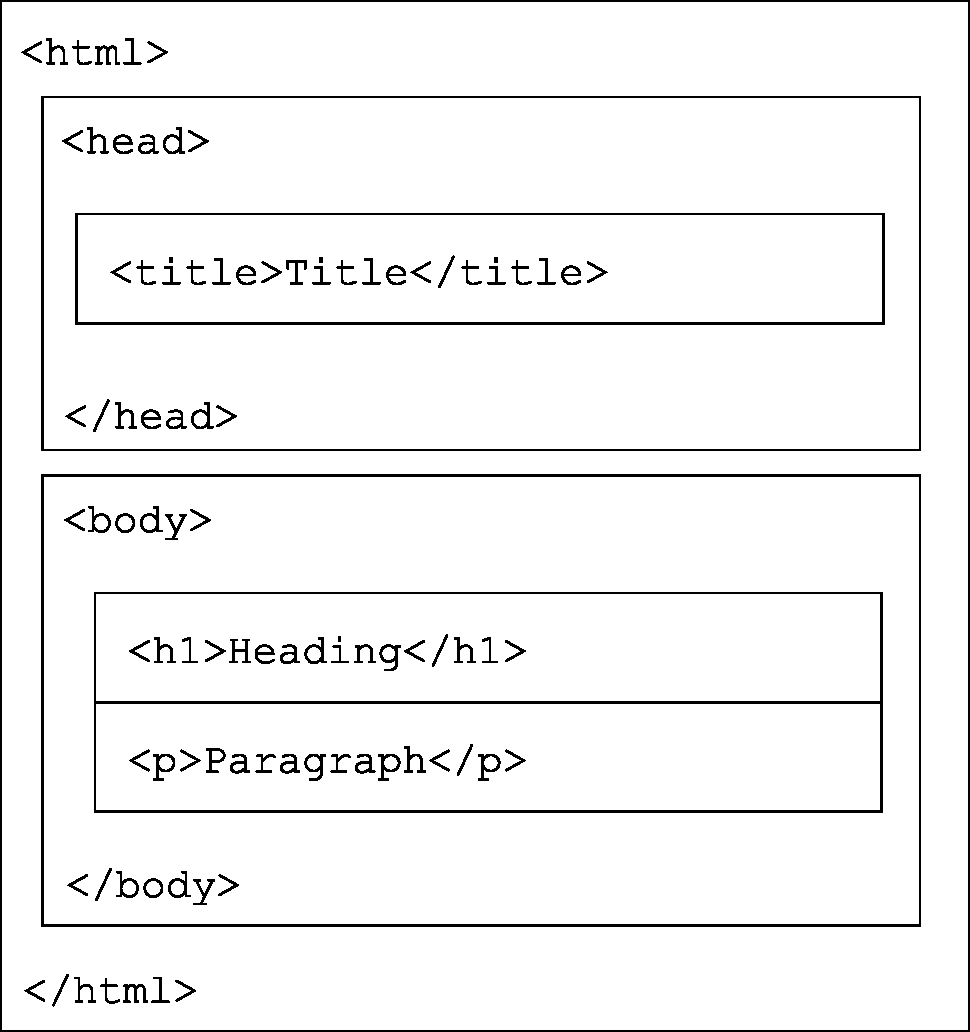
\includegraphics[keepaspectratio,width=\linewidth,height=\halfh]
    {diagrams/html-structure.pdf}

    \caption[Structure of HTML pages]{
        HTML pages are structured as a hierarchical tree of elements which enables the composition of complex structures.
        \imgcredit{Image drawn by the author of this thesis.}
    }
    \label{fig:HTMLStructure}
\end{figure}

A strong pillar of HTML's design is extensibility. There are multiple mechanisms in place to ensure applicability to a vast range of use cases. These mechanisms include:

\begin{itemize}
    \item Specifying classes of elements using the \lstinline{class} attribute. This effectively creates custom elements while still basing them on the most related, already existing elements.
    \item Using \lstinline{data-*} attributes to decorate elements with additional data that can be used by scripts. The HTML standard guarantees that these attributes are ignored by browsers.
    \item Embedding custom data using \lstinline{<script type="">} elements that can be accessed by scripts.
\end{itemize}


\section{Cascading Style Sheets (CSS)}

This section is not meant as a comprehensive guide to CSS but to give an overview and reiterate over the concepts that are important in the context of this thesis. In particular, the history of CSS is briefly summarized, a refresher on selectors and cascades is given and the different modules of CSS-based layouting are compared.

Cascading Style Sheets (CSS) is a style sheet language that is used to specify the presentation of HTML documents. It can either be embedded directly in HTML documents using \lstinline{<style>} elements or it can be defined externally and linked into them using \lstinline{<link>} elements. This characteristic of being able to externally describe the presentation of documents yields a lot of flexibility because multiple documents with different content can reuse the same presentation by linking to the same CSS file. This solved the problem of having to individually define the presentation of every page with presentation elements like \lstinline{<strong>} or \lstinline{<em>}, as was the case in earlier versions of HTML \parencite{HTML32}.

CSS was initially proposed by Håkon Wium Lie in 1994 \parencite{CSSProposal} and standardized into CSS1 by the W3C in 1996 \parencite{CSS1}. Throughout its history, the adoption of CSS by browser vendors was fraught with complications and even though most major browsers soon supported almost the full CSS standard, their implementations sometimes behaved vastly different than their competitor's. This meant that authors of web pages usually had to resort to workarounds and provide different style sheets for different browsers. In recent years, CSS specifications have become much more detailed \parencite{CSS21} and browser implementations have become more stable with less inconsistencies. It has therefore become much rarer that browser-specific workarounds have to be applied, which drastically improves the development experience.

A CSS style sheet contains a collection of rules and each rule consists of a selector and a block of style declarations. Selectors are defined in a custom syntax and are used to match HTML elements. All elements that are matched by the selector of a rule will have the rule's style declarations applied on them. The selector syntax is fairly simple when merely selecting elements of a certain type but it also provides the means for selecting elements based on their contexts or attributes. For a summary of the CSS 2.1 selector syntax, see Table \ref{tab:CSSSelectorSyntax}.

\begin{table}[tp]
    \centering
    \begin{tabularx}{\linewidth}{| l | X |}
        \hline
        \textbf{Pattern} & \textbf{Matches}                                                                  \\ \hline
        *                & Any element.                                                                      \\ \hline
        E                & Elements of type E.                                                               \\ \hline
        E F              & Any element of type F that is a descendant of elements of type E.                 \\ \hline
        E > F            & Any element of type F that is a direct descendant of elements of type E.          \\ \hline
        E + F            & Any element of type F that is a directly preceded by a sibling element of type E. \\ \hline
        E:P              & Elements of type E that also have the pseudo class P.                             \\ \hline
        .C               & Elements that have the class  C.                                                  \\ \hline
        \#I              & Elements that have the id I.                                                      \\ \hline
        [A]              & Elements that have an attribute A.                                                \\ \hline
        [A=V]            & Elements that have an attribute A with a value of V.                              \\ \hline
        S1, S2           & Elements that match either the selector S1 or the selector S2.                    \\ \hline
    \end{tabularx}
    \caption[CSS 2.1 Selector Syntax]
    {
        A summary of the CSS 2.1 selector syntax.
        \imgcredit{Table created by the author of this thesis with data from \parencite{CSS21}}
    }
    \label{tab:CSSSelectorSyntax}
\end{table}

Another important characteristic of CSS is the cascading of styles. There's a lot of depth to how the final style of an element is calculated and \cite{CSS21} should be consulted for detailed notes on this topic. The most important thing to state in the context of this work, is that styles can be overwritten. When multiple rules match an element and define different values for the same style property, the values of the rule with higher specificity will be applied. If multiple rules have the same specificity, the one defined last in the document tree will overwrite all previous ones.

\subsection{Box Layout}

All elements in a HTML document are laid out as boxes, which is defined as the CSS box model. The box model states that every element is wrapped in a rectangular box and every box is described by its content and the optional surrounding margin, border and padding areas. Margins are used to specify the invisible spacing between boxes, whereas the border is meant as a visible containment around the content of a box and the padding describes the invisible spacing between the content and the border. A visual representation of these concepts can be seen in Figure \ref{fig:BoxModel}.

\begin{figure}[tp]
    \centering
    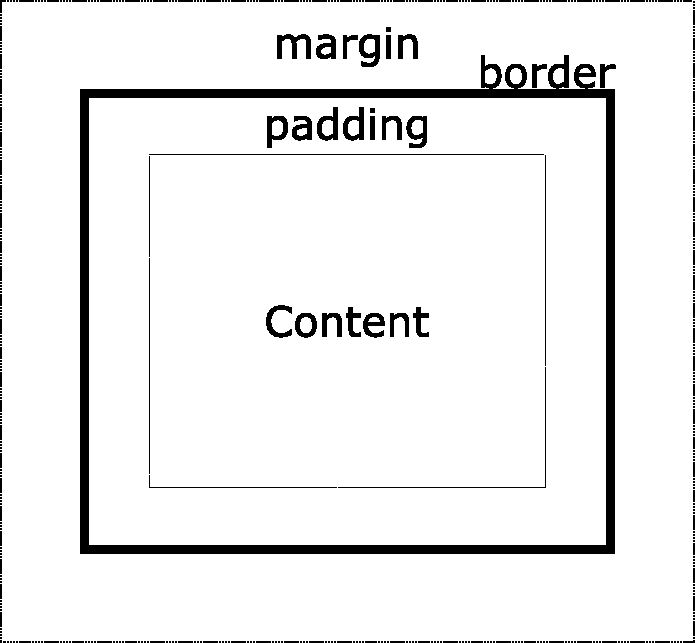
\includegraphics[keepaspectratio,width=\linewidth,height=\fullh / 3]
    {diagrams/box-model.pdf}

    \caption[CSS Box Model]{
        The CSS box model is used to define the properties of boxes that wrap around HTML elements.
        \imgcredit{Image drawn by the author of this thesis.}
    }
    \label{fig:BoxModel}
\end{figure}

In early versions of CSS, before the introduction of the Flexible Box Layout (Flexbox) Module \parencite{CSSFlexboxFirstDraft}, the box model was the only way to lay out elements. Style sheet authors had to meticulously define margins of elements and their relative (or absolute) positions in the document tree. The responsive capabilities of this kind of layouting are very limited because different configurations for varying screen sizes have to be done manually using media queries and more complex features, like filling the remaining space available, had to be implemented via scripting.

\subsection{Flexible Box Layout (Flexbox)}

Even though the first draft of the Flexbox Layout Module was already published in 2009 \parencite{CSSFlexboxFirstDraft}, browser implementations have been a slow and bug ridden process \parencite{CanIUseCSSFlexbox} that held back adoption by users for the first couple of years after its inception. Over the past few years, partly through the deprecation of Internet Explorer \parencite{IEDeprecation}, all major browser implementations of current Flexbox standards \parencite{CSSFlexbox} have become stable and, in most cases, fallback styling is not necessary anymore.

Flexbox is a mechanism for one-dimensionally laying out elements in either rows or columns. This one-dimensionality is what separates it from grid-based layouting, which is inherently two-dimensional. Flexbox layouting can be enabled for child elements via setting the \lstinline{display: flex} property on a container element. The direction of the layout can then be specified using the \lstinline{flex-direction} property which can be set to either \lstinline{row} or \lstinline{column}.

The items inside a Flexbox container can have either a fixed or a relative size. When items should be sized relative to the size of their containers, the proportions of how the available space should be divided can be controlled using ratios. These ratios can be set on item elements via the \lstinline{flex} property.

Another important feature of Flexbox layouting is the controllable spacing of items which can be specified separately for both the main and the cross axis of the layout. Spacing along the main axis can be configured with the \lstinline{justify-content} property which can take a number of different values that are demonstrated in Figure \ref{fig:FlexboxJustifyContent}. The property that controls alignment of items on the cross axis is either the \lstinline{align-items} property on container elements or the \lstinline{align-self} property on the items themselves.

\begin{figure}[tp]
    \centering
    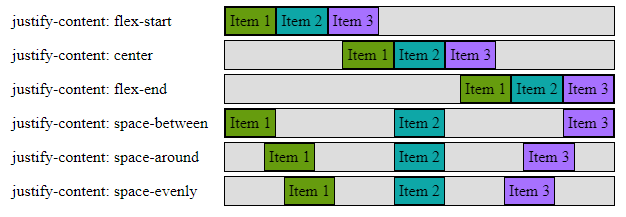
\includegraphics[keepaspectratio,width=\linewidth,height=\fullh / 3]
    {images/flexbox-justify-content.png}

    \caption[Flexbox Justify Content Property]{
        The \lstinline{justify-content} property is used to distribute items along the main axis of a Flexbox container.
        \imgcredit{Image created by the author of this thesis.}
    }
    \label{fig:FlexboxJustifyContent}
\end{figure}

This section only graced the surface of what is possible with the Flexbox Layout Module. Those properties that were discussed, were only discussed in a very broad sense and there are many useful properties like \lstinline{flex-grow}, \lstinline{flex-shrink} or \lstinline{flex-wrap} that weren't included in this overview. For a more detailed look at this topic it is recommended to review \cite{CSSFlexbox}.

\subsection{Grid Layout}

\section{JavaScript (JS)}

\section{TypeScript (TS)}

\section{Web Graphics}

\subsection{Raster Images}

\TODO{Describe raster images}

\TODO{Mention JPEG}

\TODO{Mention PNG}

\subsection{Scalable Vector Graphics (SVG)}

\TODO{Define detail in which to write about SVG}

\TODO{Describe SVG}

\TODO{Describe filters}

\TODO{Talk about issues with using CSS for styling}



SVG elements can be styled with CSS which is highly convenient as it brings all the benefits of CSS like allowing users to override parts of the styling in their own style sheets. SVG styles defined as CSS can also be animated using CSS animations and transitions. This is recommendable to manual animations using JavaScript because external configuration is inherently supported and the declarative syntax of CSS animations is powerful enough to define complex animations.

% However, SVG 1.1 \TODO{Cite spec} only supports configuration of presentation attributes via CSS and it is not possible to . Other types of attributes, like geometric attributes, can't be styled using CSS and require actual configuaration via HTML attributes. SVG 2 will support styling and animating non-presentation attributes with CSS. \TODO{Add (partial?) list of presentation attributes}\TODO{Add (partial?) list of presentation attributes}

% https://css-tricks.com/svg-properties-and-css/#svg-2
% https://stackoverflow.com/a/14258103


\subsection{Canvas}

\subsection{WebGL}

\section{Layout Engines}

\subsection{Yoga Layout}
\subsection{FaberJS}

\section{Visualization Libraries}

\subsection{Chartist}
\subsection{Highcharts}
\subsection{ECharts}
\subsection{...?}
\subsection{D3}
\TODO{Mention that D3 is successor of Protovis}

\section{Tools}
\subsection{Node}
\subsection{Rollup}
\subsection{Gulp}

